\documentclass{article}
\usepackage{graphicx}
\usepackage{amsfonts}

% Helpful vector shortcuts
\newcommand{\pderiv}[2]{\frac{\partial #1}{\partial #2}}
\newcommand{\deriv}[2]{\frac{d#1}{d#2}}
\newcommand{\crossprod}[6]{\left| \begin{array}{ccc} \hat{i} & \hat{j} & \hat{k} \\ #1 & #2 & #3 \\ #4 & #5 & #6 \end{array}\right|}
\newcommand{\curlcrossprod}[3]{\crossprod{\pderiv{}{x}}{\pderiv{}{y}}{\pderiv{}{z}}{#1}{#2}{#3}}
\newcommand{\vecx}{\vec{x}}
\newcommand{\vecb}{\vec{b}}
\newcommand{\vecr}{\vec{r}}
\newcommand{\vecz}{\vec{z}}
\newcommand{\vecp}{\vec{p}}
\newcommand{\vecomega}{\vec{\omega}}
\newcommand{\laplace}{\nabla^2}
\newcommand{\curl}{\nabla\times}
\newcommand{\colvec}[3]{\left(\begin{array}{c} #1 \\ #2 \\ #3 \end{array}\right)}
\newcommand{\dotgrad}{\cdot\nabla}

% macros to typeset code
\newcommand{\pkeyword}[1]{\textbf{#1 }}
\newcommand{\pwhile}{\pkeyword{while}}
\newcommand{\pif}{\pkeyword{if}}
\newcommand{\pthen}{\pkeyword{ then}}
\newcommand{\pelse}{\pkeyword{ else}}
\newcommand{\pindent}{\textrm{\quad}}
\newcommand{\pcomment}[1]{\textrm{#1}}
\newcommand{\pfor}{\pkeyword{for}}


\title{Incomplete Cholesky Preconditioner}
\author{Andrew Selle, Ron Fedkiw}

\begin{document}
\maketitle
\section{Preconditioned Conjugate Gradient}

For more detail on PCG see \emph{Matrix Computations}, Golub and Van Loan pg. 534 (section 10.3.1).  We wish to solve $A\vecx=\vecb$. Instead we'll
solve $\tilde{A}\tilde{\vecx}=\tilde{\vecb}$ which we call our preconditioned system.  The idea is to select a $C$ that looks like $A$.  Then we
could solve $C^{-1}A\vecx=C^{-1}\vecb$. Obviously, if $C=A$ then $A^{-1}A\vecx=I\vecx=\vecx=\vecb$. Instead, so we can simplify the actual algorithm,
we choose $\tilde{A}=C^{-1}AC^{-1}$ and $\tilde{\vecx} =C\vecx$ and $\tilde{\vecb}=C^{-1}b$. We want $\tilde{A}$ to be symmetric positive definite
like $A$. Golub defines $M=C^2=A$ as a ``preconditioner'' matrix. Note that $C=$``$\sqrt{A}$'' exists because $A$ is symmetric positive definite.

The algorithm assumes that $\vecb$ is zero in the null space, which makes sense because $b$ is in the range of $Ax$. PCG can do this by simply
reprojecting  with \verb|Enforce_Compatibility|, but this is not the best way. \verb|PROJECTION| can be smarter about this in the case of fluids, for
example handling Neumann sub-regions by adjusting only elements on the boundaries. Note that $\vecx$ may have a null space component, since PCG never
uses $\vecx$ directly. It is only used to compute $\vecr=\vecb-A\vecx$ where $A$ kills that part of $\vecx$. In fact the only place where the null
space component can return is from the solve of $M\vecz=\vecr$ and that is why we explicitly reproject it after that solve.
$$\begin{array}{ll}
k=1\\
\vecr=\vecb -A\vecx  & \\
\pwhile \|\vecr\|_\infty > \varepsilon & \\
\pindent \pkeyword{solve} M\vecz=\vecr & \pcomment{$M$ is incomplete
cholesky factor $LL^T\vecz=\vecr$}\\
\pindent\pcomment{Project out null space component of $z$}&
\\
\pindent\pif k=1 \pthen \beta=0 \pelse \beta=\vecr_{k-1}\cdot\vecz_{k-1}/\vecr_{k-2}\cdot\vecz_{k-2}&\\
\pindent \vecp_k=\vecz_{k-1}+\beta_k\vecp_{k-1}&\\
\pindent \alpha_k=\vecr_{k-1}^T\vecz_{k-1}/\vecp_k^TA\vecp_k&\\
\pindent \vecx_k=\vecx_{k-1}+\alpha_k \vecp_k\\
\pindent \vecr_k=\vecr_{k-1}-\alpha_kA\vecp_k\\
\pindent k=k+1\\
\end{array}$$
\section{Incomplete Cholesky Factorization}
Besides ``looking like'' $A$, the ``preconditioner'' $M$ should also be easy to form and invert.  Cholesky factorization produces $LL^T=LU=M$ which
can be solved by two cycles of back substitution. The algorithm as in Golub and Van Loan pg. 145 define outer product version:
$$\begin{array}{ll}
\pfor k=1:n\\
\pindent A(k,k)=\sqrt{A(k,k)}\\
\pindent A(k+1:n,k)=A(k+1:n,k)/A(k,k)\\
\pindent\pfor j=k+1:n\\
\pindent\pindent A(j:n,j)=A(j:n,j)-A(j:n,k)A(j,k)\\
\end{array}$$
Incomplete cholesky only writes to an element $i,j$ if $A(i,j)$ is non-zero.  Thus the incomplete Cholesky factorization is formed by:
$$\begin{array}{ll}
\pfor k=1:n\\
\pindent A(k,k)=\sqrt{A(k,k)}\\
\pindent \pfor i=k+1:n \\
\pindent \pindent \pif A(i,k) \ne 0 \pthen A(i,k)=A(i,k)/A(k,k)\\
\pindent\pfor j=k+1:n\\
\pindent\pindent\pfor i=j:n\\
\pindent\pindent\pindent \pif A(i,j)\ne 0 \pthen
A(i,j)=A(i,j)-A(k,i) A(j,k)\\
\end{array}$$
After the $k$th iteration of the matrix we get a $L_0L_0^T$ block like
%$$\choleskyblock{\sqrt{A(1,1)}}{}{}{}$$
$$M=L_0L_0^T=\left(\begin{array}{c|c}
\sqrt{a(k,k)} & 0 \\
\hline \begin{array}{c} \frac{a_{k+1,k}}{\sqrt{a_{k,k}}} \\ \frac{a_{k+2,k}}{\sqrt{a_{k,k}}} \\
\vdots
\\ \frac{a_{n,k}}{\sqrt{a_{k,k}}}
\end{array} & A_{k+1,k+1}-\frac{col_k col_k^T}{a_{k,k}}
 \\
\end{array}\right)
\left(\begin{array}{c|c}
\sqrt{a(k,k)} & \begin{array}{cccc} \frac{a_{k,k+1}}{\sqrt{a_{k,k}}} &\frac{a_{k,k+2}}{\sqrt{a_{k,k}}} & \cdots &  \frac{a_{k,n}}{\sqrt{a_{k,k}}}\end{array} \\
\hline 0 & A_{k+1,k+1}-\frac{col_k col_k^T}{a_{k,k}}
 \\
\end{array}\right)$$
But we would rather not compute the square root because it is expensive.  So instead of $L_0L_0^T$ for our preconditioner we will refactor it to be
$LU$ where $L=\frac{1}{\sqrt{a_{k,k}}}L_0$ and $U=\sqrt{a_{k,k}}L_0$ so we get:
$$M=LU=\left(\begin{array}{c|c}
1 & 0 \\
\hline \begin{array}{c} \frac{a_{k+1,k}}{{a_{k,k}}} \\ \frac{a_{k+2,k}}{{a_{k,k}}} \\
\vdots
\\ \frac{a_{n,k}}{{a_{k,k}}}
\end{array} & A_{k+1,k+1}-\frac{col_k col_k^T}{a_{k,k}}
 \\
\end{array}\right)
\left(\begin{array}{c|c}
{a(k,k)} & \begin{array}{cccc} a_{k,k+1} &a_{k,k+2} & \cdots &  a_{k,n}\end{array} \\
\hline 0 & A_{k+1,k+1}-\frac{col_k col_k^T}{a_{k,k}}
 \\
\end{array}\right)$$
\subsection{Uniform Grid}

For the case of the uniform grid this new factorization can be made fast. In particular, we know that we will not update for any part of the matrix
that is not in the block $A(k:n,k:n)$. In particular, the coupling associated with the bottom and with the left are not in the block. That implies
that the column and row used in the outer product will consist of only two nonzero entries, the right and the top. Thus, the only place where the
outer product can be non-zero is at these positions (the crossings in the figure). But, the crossings on the off-diagonals are zero entries in the
original matrix because right and top are decoupled so they will not be filled.  This is not true in the general case (like for an octree grid), but
in the uniform grid case it allows us to update only the diagonals. Alternatively, we can think of the reverse and consider which elements can modify
a given diagonal.  In that case only the left and bottom will modify a given cell's diagonal entry.

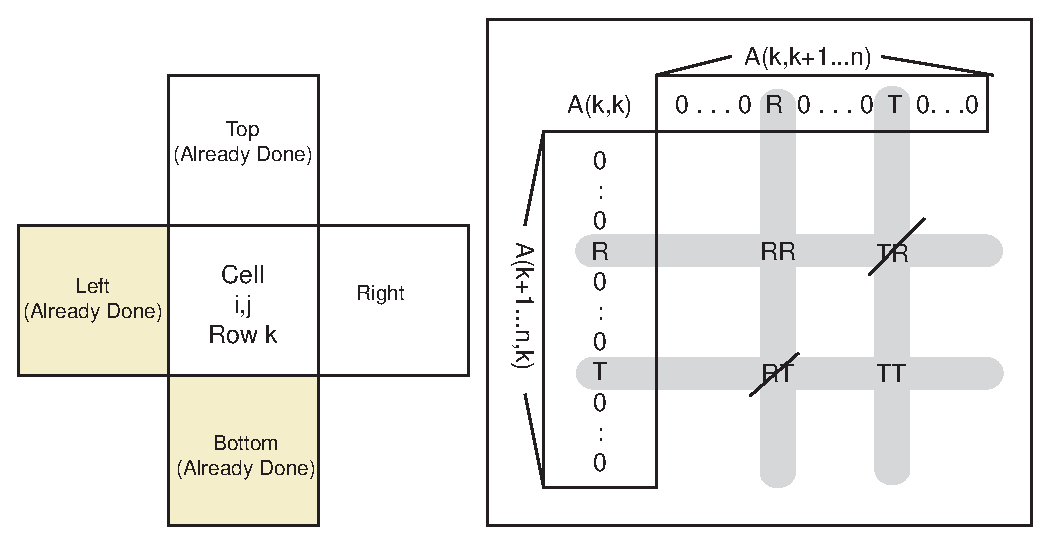
\includegraphics[width=4in]{uniform}

We can represent both $L$ and $U$ in one $n\times n$ matrix because $L$'s diagonal is all ones. For efficiency we actually represent the diagonal of
the Cholesky factorization as the reciprocal.  Note $C_\textrm{r}$, $C_\textrm{c}$, $C_\textrm{t}$ are the right, center, and top values for a given
matrix row for the cell $i,j$. The code to form the $LU$ matrices for 2d becomes:
$$\begin{array}{ll}
C=A\\
\pfor k=1:n\\
\pindent i,j\in\mathbb{Z^+} \textrm{ \quad s.t. } k=i+jN\\
\pindent 1/[C_\textrm{c}(i,j)=A(k,k)-C_\textrm{r}(i-1,j)^2 C_\textrm{c}(i-1,j) -C_\textrm{t}(i,j-1)^2C_\textrm{c}(i,j-1)]\\
\end{array}$$

When doing the backsubstitution solves during the $Mz=b$ step of PCG, we see that having the reciprocal diagonal allows us to multiply instead of
divide by the diagonal element during a row solve.


\subsection{Sparse Matrix}

In a general sparse matrix we cannot make the simplifying assumption of only modifying the diagonal.  Moreover the representation of the sparsity
biases certain accesses to be computationally cheaper.  Our implementation keeps each row of the matrix in a sparse vector which keeps an array of
indices and values. Thus, traversing the columns of a single row is very cheap.  Traversing down a column is expensive. Thus, we reorder the Cholesky
formation process to only go through each row once.

\subsection{Modified Cholesky}

Incomplete Cholesky is known to perform poorly as the grid is refined.  To solve this problem, the modified Cholesky scheme is employed, where the
elements of the outer product that are not filled in (due to the sparsity pattern of $A$) are added to diagonal of that row instead - usually
diminished by a factor of about $.95$.

$$\begin{array}{ll}
\pfor k=1:n\\
\pindent A(k,k)=\sqrt{A(k,k)}\\
\pindent \pfor i=k+1:n \\
\pindent \pindent \pif A(i,k) \ne 0 \pthen A(i,k)=A(i,k)/A(k,k)\\
\pindent\pfor j=k+1:n\\
\pindent\pindent\pfor i=j:n\\
\pindent\pindent\pindent\,\, \pif\ A(i,j)\ne 0 \pthen
A(i,j)=A(i,j)-A(k,i) A(j,k)\\
\pindent\pindent\pindent\pelse\ A(i,i)=A(i,i)-A(k,i)A(j,k)\\
\end{array}$$
More detail can be found in Chan and Van Der Vorst \emph{Approximate and Incomplete Factorizations}.

\end{document}
